\section{Evaluation Settings}
\label{app:eval_details}

This section provides comprehensive configuration details and testing protocols for all benchmarks reported in Table~\ref{tab:instruct_eval}.

\subsection{General Evaluation Protocol}
\label{app:eval_general}

Unless explicitly stated otherwise, all experiments for Kimi-K2.5 adhere to the following hyperparameter configuration:
\begin{itemize}
    \item \textbf{Temperature:} $1.0$
    \item \textbf{Top-p:} $0.95$
    \item \textbf{Context Length:} $256\text{k}$ tokens
\end{itemize}

\subsection{Baselines}
For baseline models, we report results under their respective high-performance reasoning configurations:
\begin{itemize}
    \item \textbf{Claude Opus 4.5:} Extended thinking mode
    \item \textbf{GPT-5.2:} Maximum reasoning effort (\texttt{xhigh})
    \item \textbf{Gemini 3 Pro:} High thinking level
    \item \textbf{DeepSeek-V3.2:} Thinking mode enabled (for text-only benchmarks)
    \item \textbf{Qwen3-VL-235B-A22B:} Thinking mode (for vision benchmarks only)
\end{itemize}

For vision and multimodal benchmarks, GPT-5.2-xhigh exhibited an approximate 10\% failure rate (i.e., no output generated despite three retry attempts) during vision evaluations. These failures were treated as incorrect predictions, meaning that the reported scores may be conservative lower bounds of the model’s true capability.

In addition, because we were unable to consistently access a stable GPT-5.2 API, we skipped some benchmarks with high evaluation costs, such as WideSearch.

\subsection{Text Benchmarks}
\label{app:eval_text}



\paragraph{Reasoning Benchmarks.}
For high-complexity reasoning benchmarks, including HLE-Full, AIME 2025, HMMT 2025, GPQA-Diamond, and IMO-AnswerBench, we enforce a maximum completion budget of $96\text{k}$ tokens to ensure sufficient reasoning depth. To reduce variance arising from stochastic reasoning paths, results on AIME 2025 and HMMT 2025 (Feb) are averaged over 64 independent runs (Avg@64), while GPQA-Diamond is averaged over 8 runs (Avg@8).

\paragraph{LongBench v2.}\label{app:eval_longcontext}
For a fair comparison, we standardize all input contexts to approximately $128\text{k}$ tokens using the same truncation strategy as in~\cite{bai2025longbenchv2deeperunderstanding}.
We observe that GPT5.2-xhigh frequently produces free-form question--answer style responses rather than the required multiple-choice format.
Therefore, we report results using GPT5.2-high, which consistently adheres to the expected output format.

\subsection{Image and Video Benchmarks}
\label{app:eval_vision}

All image and video understanding evaluations utilize the following configuration:
\begin{itemize}
    \item \textbf{Maximum Tokens:} $64\text{k}$
    \item \textbf{Sampling:} Averaged over 3 independent runs (Avg@3)
\end{itemize}


\paragraph{ZeroBench (w/ tools).} Multi-step reasoning evaluations use constrained step-wise generation:
\begin{itemize}
    \item \textbf{Max Tokens per Step:} $24\text{k}$
    \item \textbf{Maximum Steps:} $30$
\end{itemize}

\paragraph{MMMU-Pro.} We adhere strictly to the official evaluation protocol: input order is preserved for all modalities, with images prepended to text sequences as specified in the benchmark guidelines. 

\paragraph{Sampling Strategies for Video Benchmarks.} For short video benchmarks (VideoMMMU, MMVU \& MotionBench), we sample 128 uniform input frames with a maximum spatial resolution at 896; 2048 uniform frames are sampled for long video benchmarks (Video-MME, LongVideoBench \& LVBench) with 448 spatial resolution.

\paragraph{Specialized Metrics.} 
\begin{itemize}
    \item \textbf{OmniDocBench 1.5:} Scores are computed as $(1 - \text{normalized Levenshtein distance}) \times 100$, where higher values indicate superior OCR and document understanding accuracy.
    \item \textbf{WorldVQA:} Access available at \url{https://github.com/MoonshotAI/WorldVQA}. This benchmark evaluates atomic, vision-centric world knowledge requiring fine-grained visual recognition and geographic understanding.
\end{itemize}


\subsection{Coding and Software Engineering}
\label{app:eval_coding}

\paragraph{Terminal Bench 2.0.} All scores are obtained using the default Terminus-2 agent framework with the provided JSON parser. Notably, we evaluate under \textbf{non-thinking mode} because our current context management implementation for thinking mode is technically incompatible with Terminus-2's conversation state handling.

\paragraph{SWE-Bench Series.} We employ an internally developed evaluation framework featuring a minimal tool set: \texttt{bash}, \texttt{create\_file}, \texttt{insert}, \texttt{view}, \texttt{str\_replace}, and \texttt{submit}. System prompts are specifically tailored for repository-level code manipulation. Peak performance is achieved under \textbf{non-thinking mode} across all SWE-Bench variants (Verified, Multilingual, and Pro).

\paragraph{CyberGym.} Claude Opus 4.5 results for this benchmark are reported under non-thinking settings as specified in their technical documentation. We report scores in the difficulty level 1 (the primary setting).

\paragraph{PaperBench.} We report the scores under the CodeDev setting.

\paragraph{Sampling.} All coding task results are averaged over 5 independent runs (Avg@5) to ensure stability across environment initialization and non-deterministic test case ordering.

\subsection{Agentic Evaluation}
\label{app:eval_agentic}

\paragraph{Tool Setting.} Kimi-K2.5 is equipped with web search tool, code interpreter (Python execution environment), and web browsing tools for all agentic evaluations, including HLE with tools and agentic search benchmarks (BrowseComp, WideSearch, DeepSearchQA, FinSearchComp T2\&T3 and Seal-0).

\paragraph{Context Management Strategies.} 
To handle the extended trajectory lengths inherent in complex agentic tasks, we implement domain-specific context management protocols. Unless otherwise specified below, \textbf{no context management} is applied to agentic evaluations; tasks exceeding the model's supported context window are directly counted as failures rather than truncated.

\begin{itemize}
    \item \textbf{Humanity's Last Exam (HLE).} For the HLE tool-augmented setting, we employ a \textit{Hide-Tool-Result Context Management} strategy: when the context length exceeds predefined thresholds, only the most recent round of tool messages (observations and return values) is retained, while the reasoning chain and thinking processes from all previous steps are preserved in full.
    
    \item \textbf{BrowseComp.} For BrowseComp evaluations, our evaluation contains both with and without context management settings. Under the context management setting, we adopt the same \textit{discard-all} strategy proposed by DeepSeek, where all history is truncated once token thresholds are exceeded.
\end{itemize}
\paragraph{System Prompt.} 
All agentic search and HLE evaluations utilize the following unified system prompt, where \texttt{DATE} is dynamically set to the current timestamp:

{\small
\begin{verbatim}
You are Kimi, today's date: DATE.
Your task is to help the user with their questions by using various tools, 
thinking deeply, and ultimately answering the user's questions.

Please follow the following principles strictly during the deep research:
1. Always focus on the user's original question during the research process, 
   avoiding deviating from the topic.
2. When facing uncertain information, use search tools to confirm.
3. When searching, filter high-trust sources (such as authoritative websites, 
   academic databases, and professional media) and maintain a critical mindset 
   towards low-trust sources.
4. When performing numerical calculations, prioritize using programming tools 
   to ensure accuracy.
5. Please use the format [^index^] to cite any information you use.
6. This is a **Very Difficult** problem—do not underestimate it. You must use 
   tools to help your reasoning and then solve the problem.
7. Before you finally give your answer, please recall what the question is 
   asking for.
\end{verbatim}
}

\paragraph{Sampling Protocol.} 
To account for the inherent stochasticity in search engine result rankings and dynamic web content availability, results for Seal-0 and WideSearch are averaged over 4 independent runs (Avg@4). All other agentic benchmarks are evaluated under single-run protocols unless explicitly stated otherwise.

\subsection{Computer-Use Evaluation}
\label{app:eval_computer_use}

\paragraph{Hyperparameter Settings.} We set $\texttt{max\_steps\_per\_episode}=100$ for all experiments, with $\texttt{temperature}=0$ for OSWorld-Verified and $\texttt{temperature}=0.1$ for WebArena. Due to resource constraints, all models are evaluated in a one-shot setting. Adhering to the OpenCUA configuration~\citep{wang2025opencuaopenfoundationscomputeruse}, the agent context includes the last 3 history images, the complete thought history, and the task instruction. For WebArena, we manually corrected errors in the evaluation scripts and employed $\texttt{GPT-4o}$ as the judge model for the $\texttt{fuzzy\_match}$ function. To ensure fair comparison, Claude Opus 4.5 is evaluated solely with computer-use tools (excluding browser tools), a departure from the System Card configuration~\citep{opus45report}.

\paragraph{System Prompt} We utilize a unified system prompt for all computer use tasks:
{\small
\begin{verbatim}
You are a GUI agent. You are given an instruction, a screenshot of the screen and your
previous interactions with the computer. You need to perform a series of actions to 
complete the task. The password of the computer is {password}.

For each step, provide your response in this format:
{thought}
## Action:
{action}
## Code:
{code}

In the code section, the code should be either pyautogui code or one of the following 
functions wrapped in the code block:
- {"name": "computer.wait", "description": "Make the computer wait for 20 seconds 
for installation, running code, etc.", "parameters": {"type": "object", "properties": 
{}, "required": []}}
- {"name": "computer.terminate", "description": "Terminate the current task and report
its completion status", "parameters": {"type": "object", "properties": {"status": 
{"type": "string", "enum": ["success", "failure"], "description": "The status of the 
task"}, "answer": {"type": "string", "description": "The answer of the task"}}, 
"required": ["status"]}}
\end{verbatim}
}



\subsection{Agent Swarm Configuration}
\label{app:eval_swarm}
\paragraph{Tool Setting.} In addition to the core toolset described in Appendix~\ref{app:eval_agentic} (web search, code interpreter, and web browsing), the orchestrator is equipped with two specialized tools for sub-agent creation and scheduling:

\begin{itemize}
    \item \texttt{create\_subagent}: Instantiates a specialized sub-agent with a custom system prompt and identifier for reuse across tasks.
    \item \texttt{assign\_task}: Dispatches assignments to created sub-agents.
\end{itemize}

The tool schemas are provided below:

{
\small
\begin{verbatim}
{
 "name": "create_subagent",
 "description": "Create a custom subagent with specific system prompt 
   and name for reuse.",
 "parameters": {
   "type": "object",
   "properties": {
     "name": {
       "type": "string",
       "description": "Unique name for this agent configuration"
     },
     "system_prompt": {
       "type": "string",
       "description": "System prompt defining the agent's role, 
         capabilities, and boundaries"
     }
   },
   "required": ["name", "system_prompt"]
 }
}
{
 "name": "assign_task",
 "description": "Launch a new agent.\nUsage notes:\n
   1. You can launch multiple agents concurrently whenever possible,
      to maximize performance;\n
   2. When the agent is done, it will return a single message back to you.",
 "parameters": {
   "type": "object",
   "properties": {
     "agent": {
       "type": "string",
       "description": "Specify which created agent to use."
     },
     "prompt": {
       "type": "string",
       "description": "The task for the agent to perform"
     }
   },
   "required": ["agent", "prompt"]
 }
}
\end{verbatim}
}

\paragraph{Step Limits.} When operating in Agent Swarm mode, we set computational budgets for the orchestrator and sub-agents. Step limits apply to the aggregate count of tool invocations and environment interactions.

\begin{itemize}
    \item \textbf{BrowseComp:} The orchestrator is constrained to a maximum of 15 steps. Each spawned sub-agent operates under a limit of 100 steps (i.e., up to 100 tool calls per sub-agent).
    \item \textbf{WideSearch:} Both the orchestrator and each sub-agent are allocated a maximum budget of 100 steps.
    \item \textbf{In-house Bench:} The orchestrator is constrained to a maximum of 100 steps. Each spawned sub-agent operates under a limit of 50 steps .
\end{itemize}

\paragraph{System Prompt.} 
{\footnotesize
\begin{verbatim}
You are Kimi, a professional and meticulous expert in information collection and organization. 
You fully understand user needs, skillfully use various tools, and complete tasks with the
highest efficiency.
# Task Description
After receiving users' questions, you need to fully understand their needs and think 
about and plan how to complete the tasks efficiently and quickly.
# Available Tools
To help you complete tasks better and faster, I have provided you with the following tools:
1. Search tool: You can use the search engine to retrieve information, supporting multiple 
queries in parallel.
2. Browser tools: You can visit web links (web pages, PDFs, etc.), get page content, and 
perform interactions such as clicking, inputting, finding, and scrolling.
3. Sub Agent tools:
   - `create_subagent`: Create a new sub-agent with a unique name and clear, specific 
   system prompt.
   - `assign_task`: Delegate tasks to created sub-agents. Sub-agents can also use search 
   and browser tools.
4. Other tools: Including code execution (IPython, Shell).
\end{verbatim}
}



\subsection{GDPVal}
\label{app:eval_gdpval}

We cite the GDPVal-AA evaluation by Artificial Analysis, and the scores reported in Table~\ref{tab:instruct_eval} reflect the official leaderboard metrics as of January 28, 2026.

\begin{figure}[p]
    \centering
    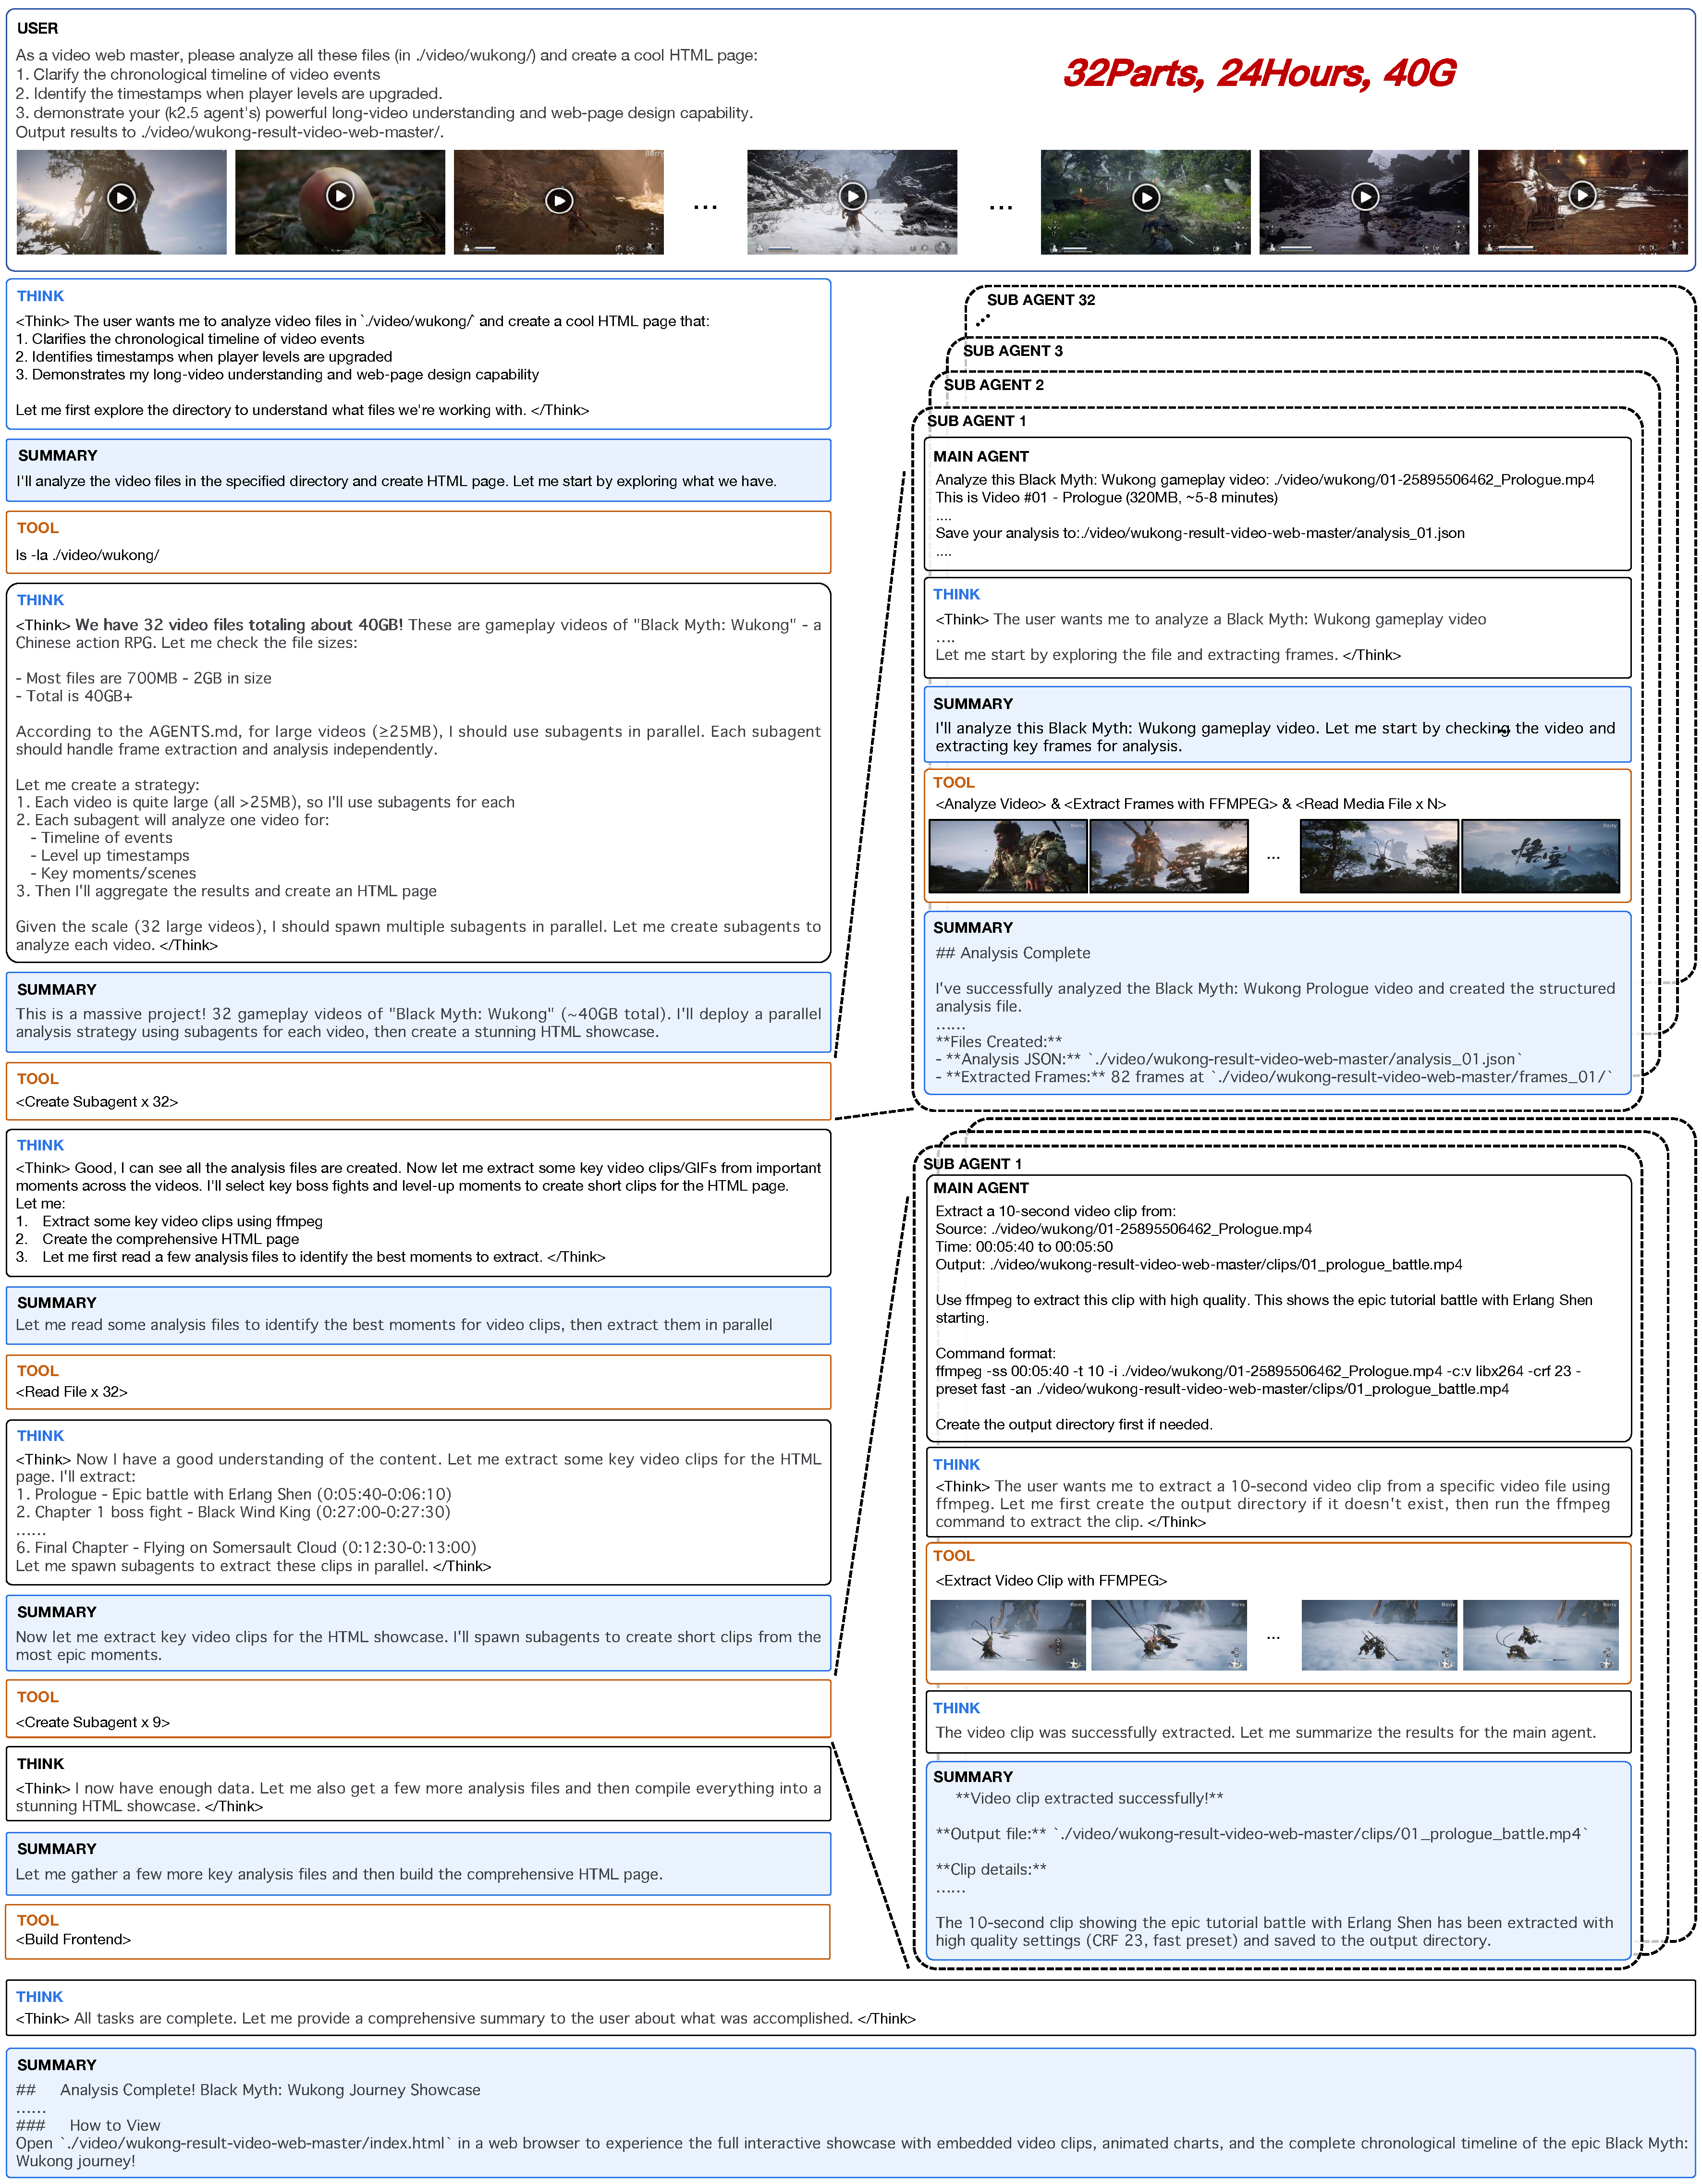
\includegraphics[width=\linewidth]{figures/video_agent_case.pdf}
    \caption{Qualitative example of Kimi K2.5 analyzing a {complete playthrough} of \textit{Black Myth: Wukong} ({24 hours} of continuous gameplay across {32 videos} at 1080p) using parallel visual agents. See \href{https://statics.moonshot.cn/k25-vibe-cases/blackmyth-wukong/index.html}{generated webpage} and \href{https://www.bilibili.com/video/BV1dbyaBZE8n/}{source videos} (all rights reserved by source authors).}
    \label{fig:video_case}
\end{figure}

\begin{figure}[p]
    \centering
    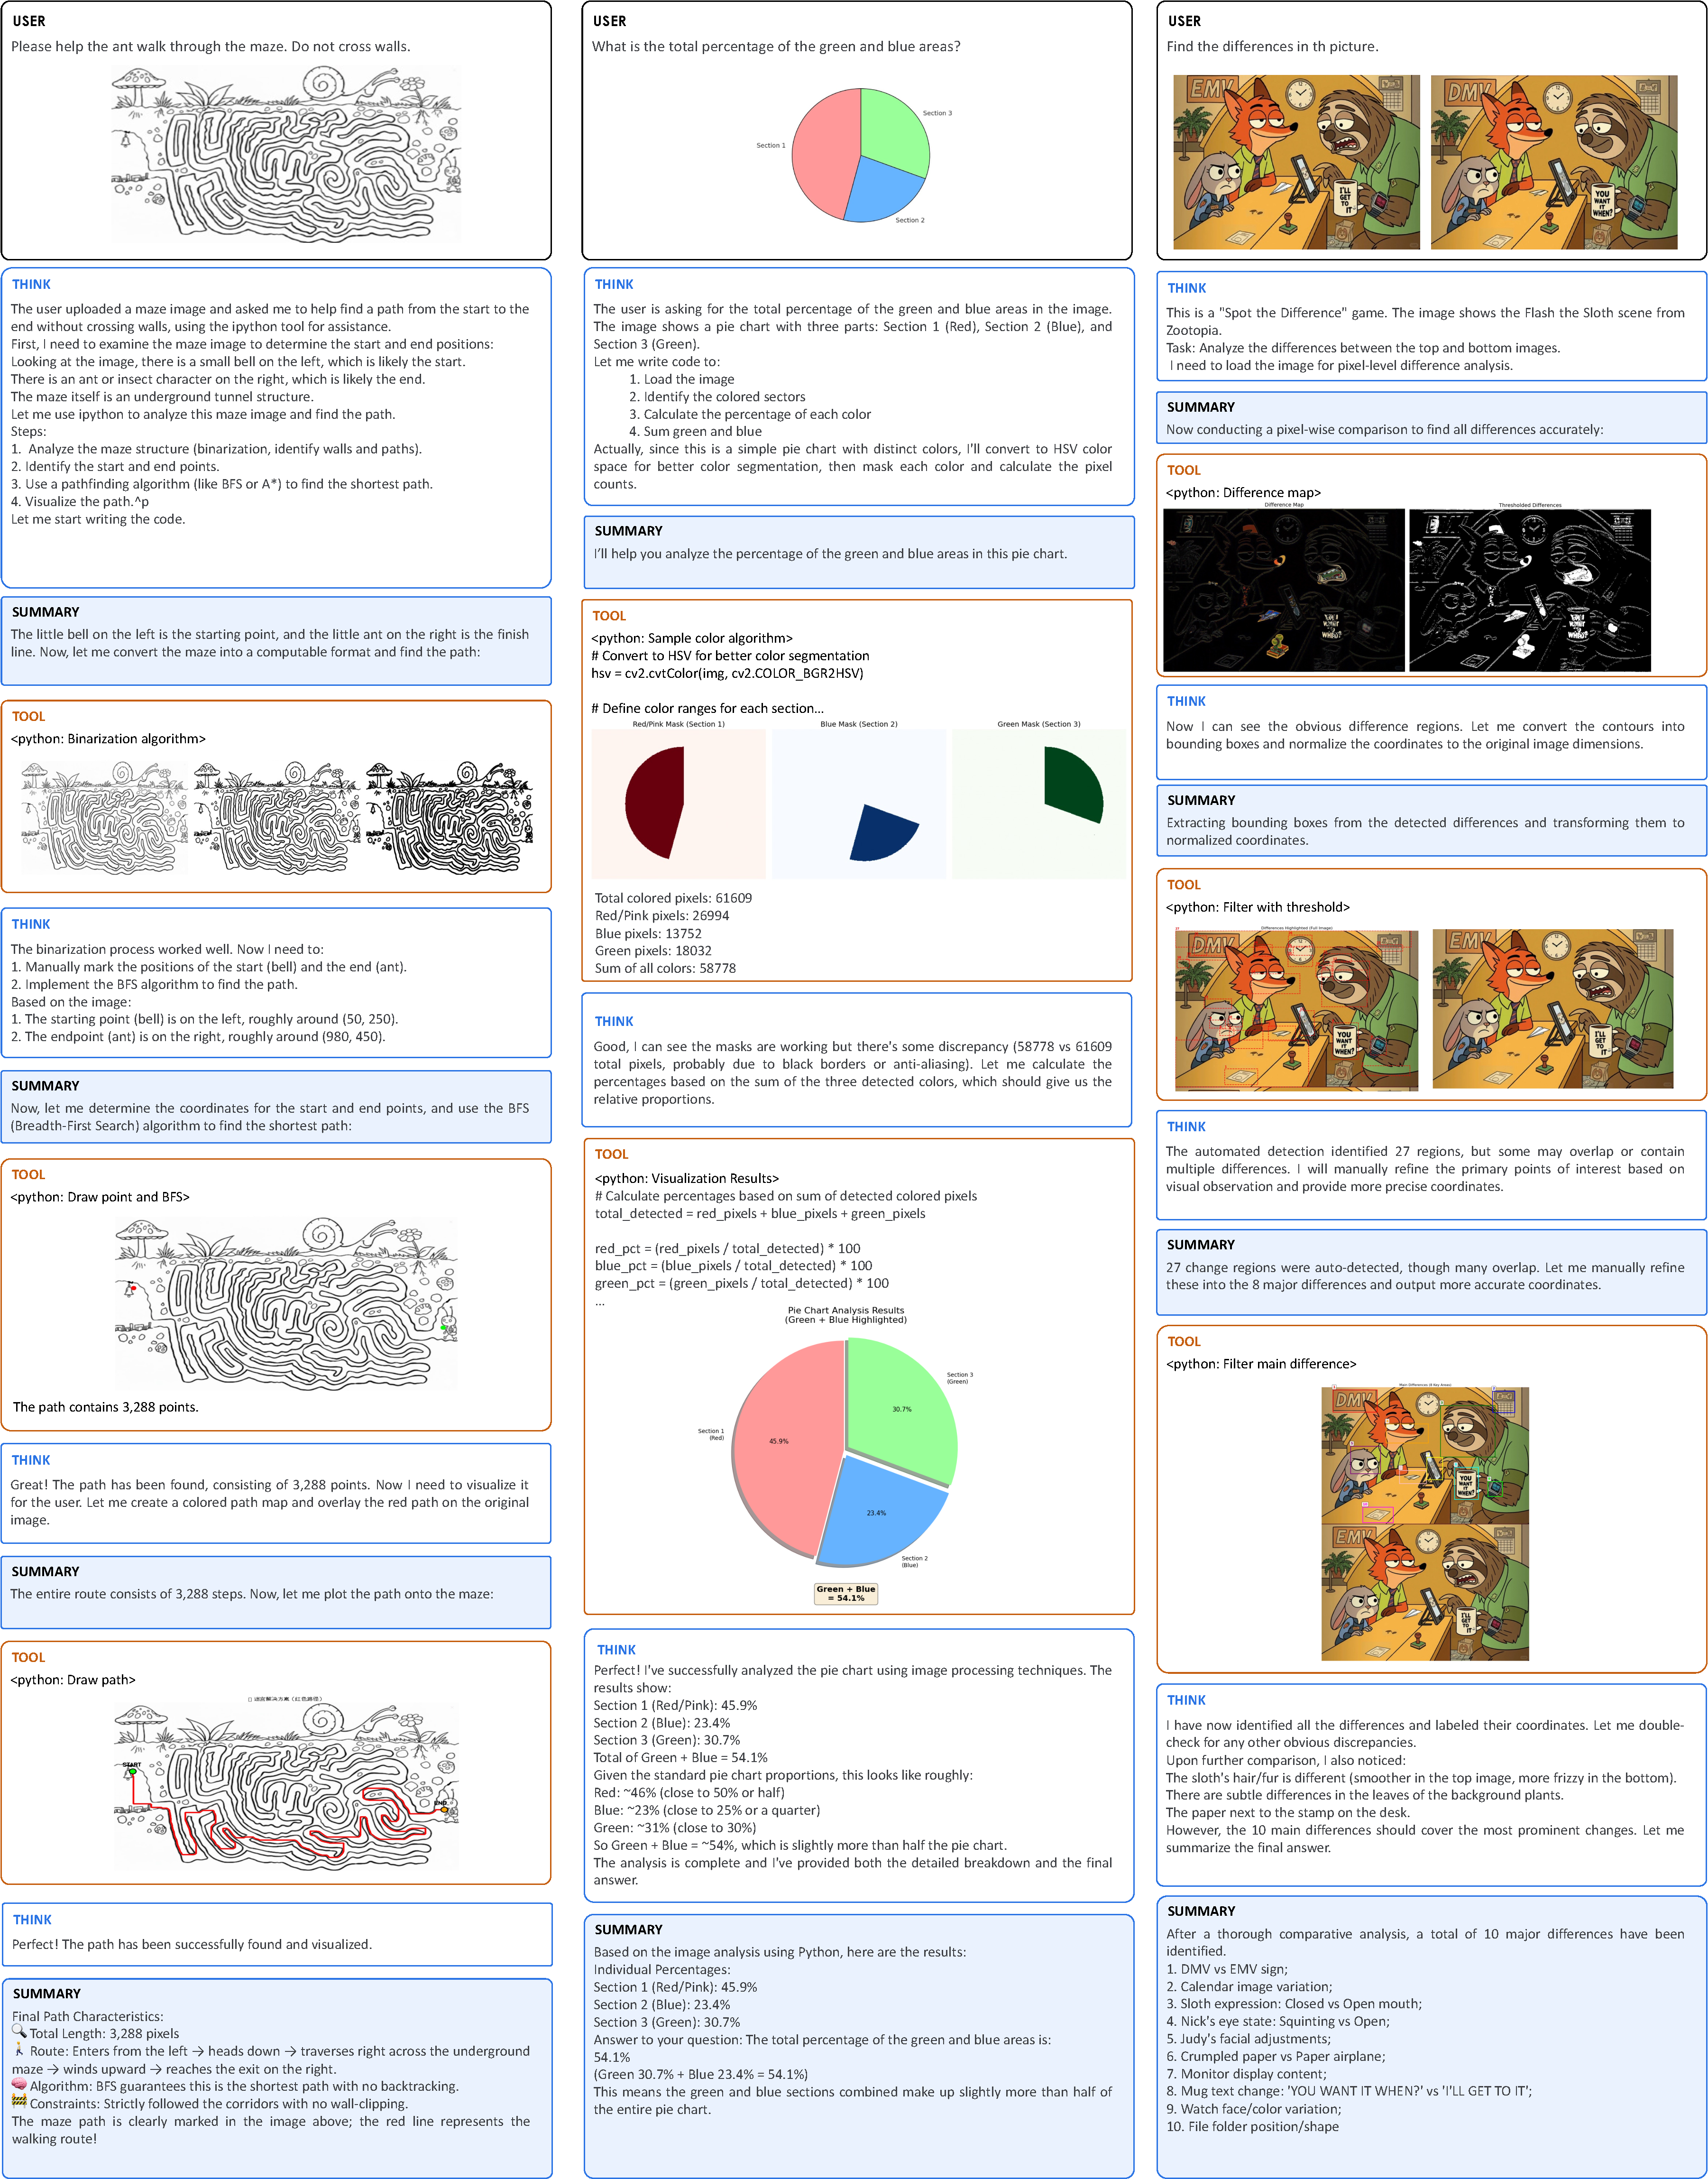
\includegraphics[width=0.96\textwidth]{figures/vtir_examples.pdf}
    \caption{Qualitative examples of Kimi K2.5 solving visual reasoning tasks via tool use.} 
    \label{fig:cases_vtir}
\end{figure}

\clearpage

\section{Visualization}

Figure~\ref{fig:video_case} demonstrates our Agent Swarm tackling a challenging long-form video understanding task: analyzing a complete playthrough of \textit{Black Myth: Wukong} (24 hours of continuous gameplay across 32 videos, totaling 40GB). The system employs a hierarchical multi-agent architecture where a Main Agent orchestrates parallel Sub Agents to process individual video segments independently. Each sub agent performs frame extraction, temporal event analysis, and key moment identification (e.g., boss fights, level-ups). The Main Agent subsequently aggregates these distributed analyses to synthesize a comprehensive HTML showcase featuring chronological timelines, embedded video clips, and interactive visualizations. This example demonstrates the system's ability to handle massive-scale multimodal content through parallelization while maintaining coherent long-context understanding.

Figure~\ref{fig:cases_vtir} presents qualitative examples of Kimi K2.5 solving diverse visual reasoning tasks via tool-augmented reasoning. The model demonstrates: \textbf{(1)} Maze Solving—processing binary image segmentation and implementing pathfinding algorithms (BFS) to navigate complex mazes; \textbf{(2)} Pie Chart Analysis—performing pixel-level color segmentation and geometric calculations to determine precise area proportions;  and \textbf{(3)} Spot-the-Difference—employing computer vision techniques to detect pixel-level discrepancies between image pairs. These examples highlight the model's capability to decompose complex visual problems into executable code, iteratively refine strategies based on intermediate results, and synthesize precise answers through quantitative visual analysis.